\section{Anhang}\label{sec:anhang}

\subsection*{Linearer Verst\"arker}

\begin{table}[ht]
  \centering
  \caption{Messwerte des 1. linearen Verstärkers.}
  \label{tab:lin_verst_01}
  \input{build/lin_verst_01__r1_200__rn_470__u1_100_data.tex}
\end{table}

\begin{table}[ht]
  \centering
  \caption{Messwerte des 2. linearen Verstärkers.}
  \label{tab:lin_verst_02}
  \input{build/lin_verst_02__r1_200__rn_100__u1_100_data.tex}
\end{table}

\begin{table}[ht]
  \centering
  \caption{Messwerte des 3. linearen Verstärkers.}
  \label{tab:lin_verst_03}
  \input{build/lin_verst_03__r1_100__rn_470__u1_100_data.tex}
\end{table}

\begin{table}[ht]
  \centering
  \caption{Messwerte des 4. linearen Verstärkers.}
  \label{tab:lin_verst_04}
  \input{build/lin_verst_04__r1_470__rn_100__u1_100_data.tex}
\end{table}

\FloatBarrier
\newpage
\subsection*{Integrator, Differentiator}

\begin{table}[ht]
  \centering
  \caption{Messwerte des Integrators.}
  \label{tab:int}
  \input{build/integrator_data.tex}
\end{table}

\begin{table}[ht]
  \centering
  \caption{Messwerte des Differentiators.}
  \label{tab:dif}
  % \sisetup{add-decimal-zero=false}
  \input{build/differentiator_data.tex}
\end{table}

\FloatBarrier
\newpage

\begin{figure}[ht]
  \centering
  \begin{subfigure}[]{\textwidth}
    \centering
    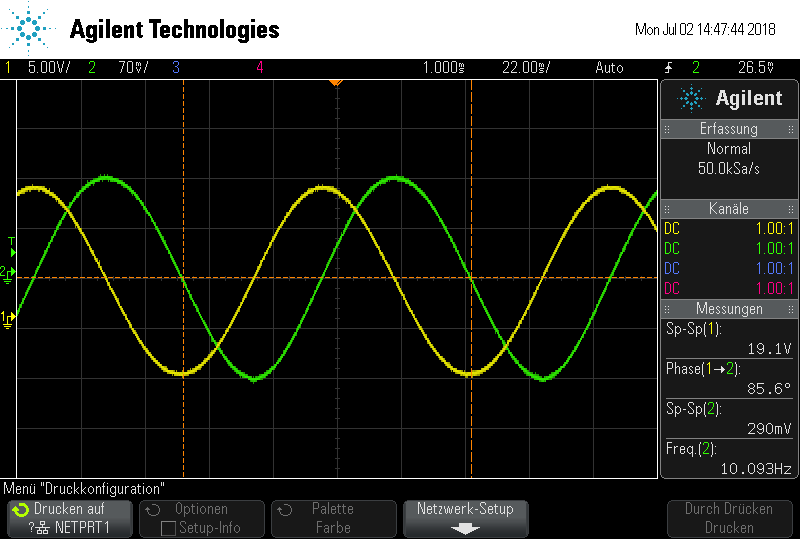
\includegraphics[height=0.28\textheight]{data/scope_262.png}
    \caption{Integration einer Sinusspannung (grün) ergibt eine Cosinusspannung (gelb).}
    \label{subfig:int_sinus}
  \end{subfigure}
  \begin{subfigure}[]{\textwidth}
    \centering
    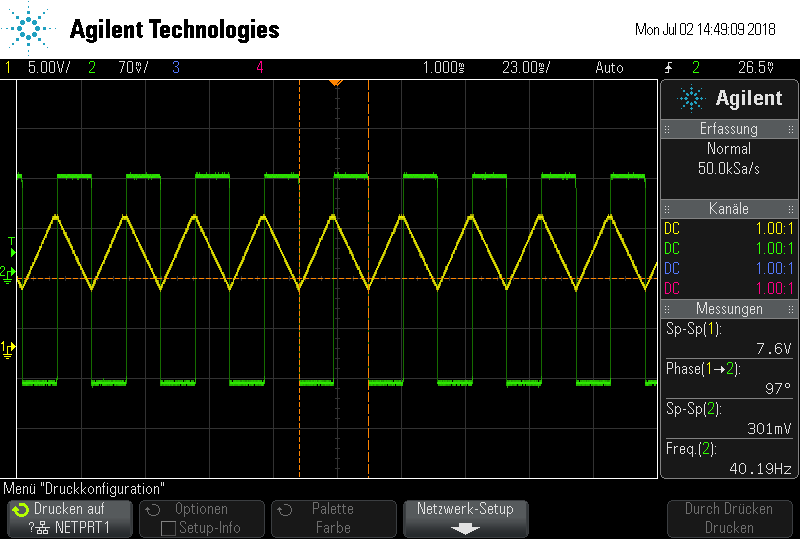
\includegraphics[height=0.28\textheight]{data/scope_263.png}
    \caption{Integration einer Rechteckspannung (grün) ergibt eine Dreieckspannung (gelb).}
    \label{subfig:int_rechteck}
  \end{subfigure}
  \begin{subfigure}[]{\textwidth}
    \centering
    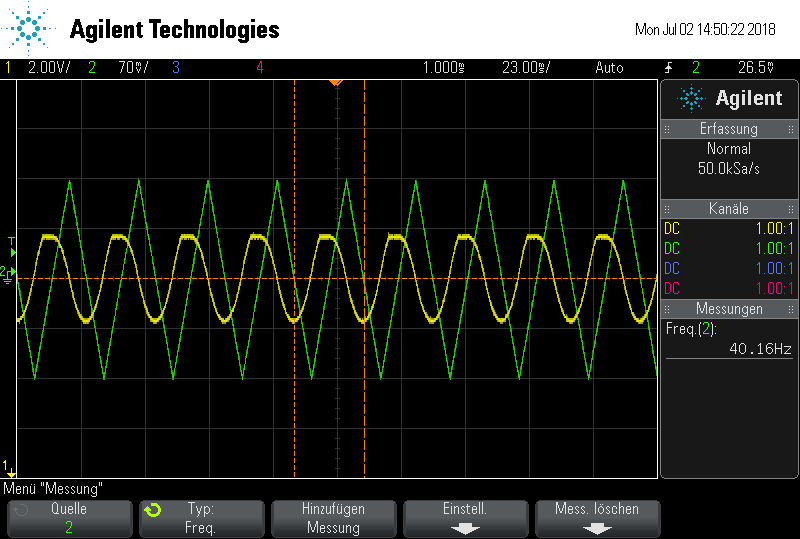
\includegraphics[height=0.28\textheight]{data/scope_264.png}
    \caption{Integration einer Dreieckspannung (grün) ergibt eine Spannung mit quadratischer
    Funktion (gelb).}
    \label{subfig:int_dreieck}
  \end{subfigure}
  \caption{Aufnahmen des Oszilloskops von verschiedenen Integrationen.}
  \label{fig:integrationen}
\end{figure}


\begin{figure}[ht]
  \centering
  \begin{subfigure}[]{\textwidth}
    \centering
    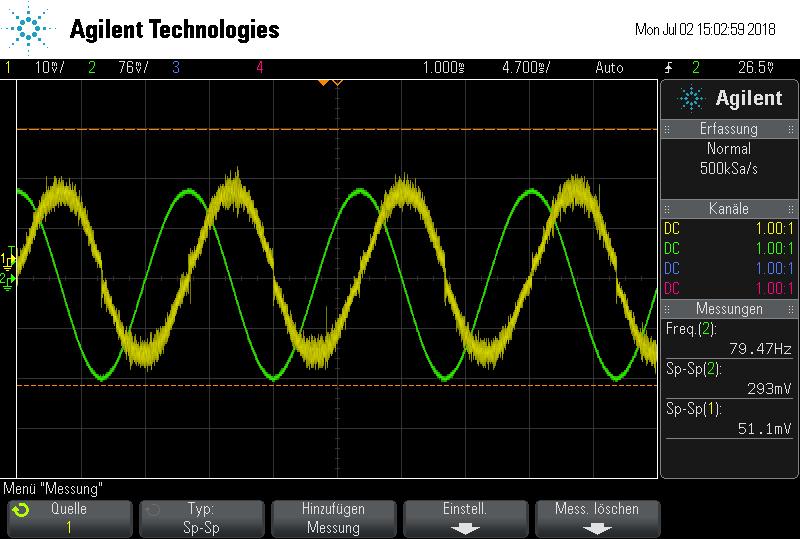
\includegraphics[height=0.28\textheight]{data/scope_265.png}
    \caption{Differentiation einer Sinusspannung (grün) ergibt eine Cosinusspannung (gelb).}
    \label{subfig:dif_sinus}
  \end{subfigure}
  \begin{subfigure}[]{\textwidth}
    \centering
    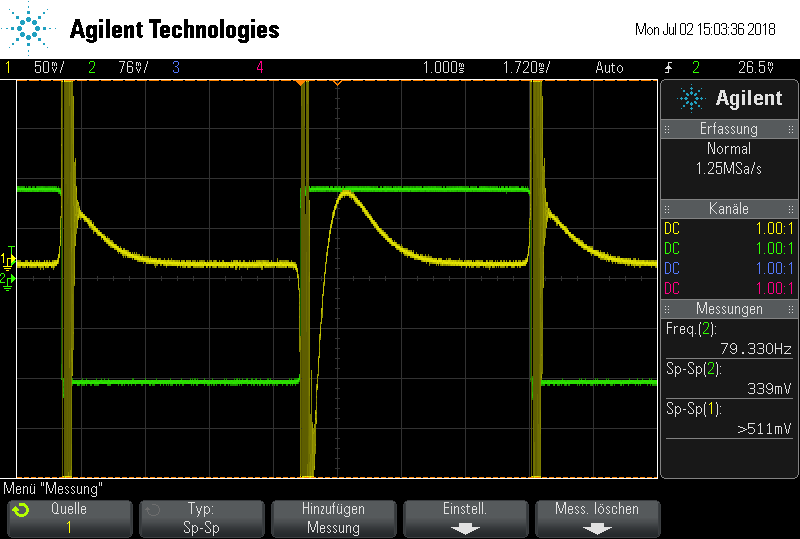
\includegraphics[height=0.28\textheight]{data/scope_266.png}
    \caption{Differentiation einer Rechteckspannung (grün) ergibt eine Delta-Distribution (gelb).}
    \label{subfig:dif_rechteck}
  \end{subfigure}
  \begin{subfigure}[]{\textwidth}
    \centering
    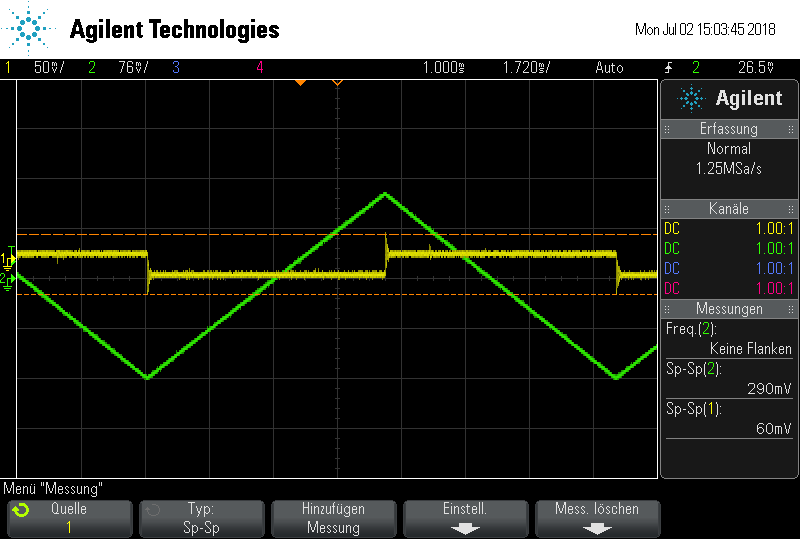
\includegraphics[height=0.28\textheight]{data/scope_267.png}
    \caption{Differentiation einer Dreieckspannung (grün) ergibt eine Rechteckspannung (gelb).}
    \label{subfig:dif_dreieck}
  \end{subfigure}
  \caption{Aufnahmen des Oszilloskops von verschiedenen Differentiationen.}
  \label{fig:differentiationen}
\end{figure}
